\documentclass[12pt]{article}

\usepackage{tabularx}
\usepackage{booktabs}
\usepackage[letterpaper, portrait, margin=1in]{geometry}
\usepackage{helvet}
\usepackage{hyperref}
\renewcommand{\familydefault}{\sfdefault}
\usepackage{afterpage}
\usepackage{titlepic}
\usepackage[dvipsnames]{xcolor}
\usepackage{graphicx}

\usepackage{titlesec}
\titleformat{\section}{\large\bfseries\color{RedOrange}}{\rlap{\color{black}\rule[-0.3cm]{\linewidth}{1cm}} {\textcolor{RedOrange}{\thesection}}}{1em}{}
\usepackage[none]{hyphenat} 
\usepackage{longtable}

\title{\textbf{Problem Statement and Goals\\\progname \\ \vspace{2cm} 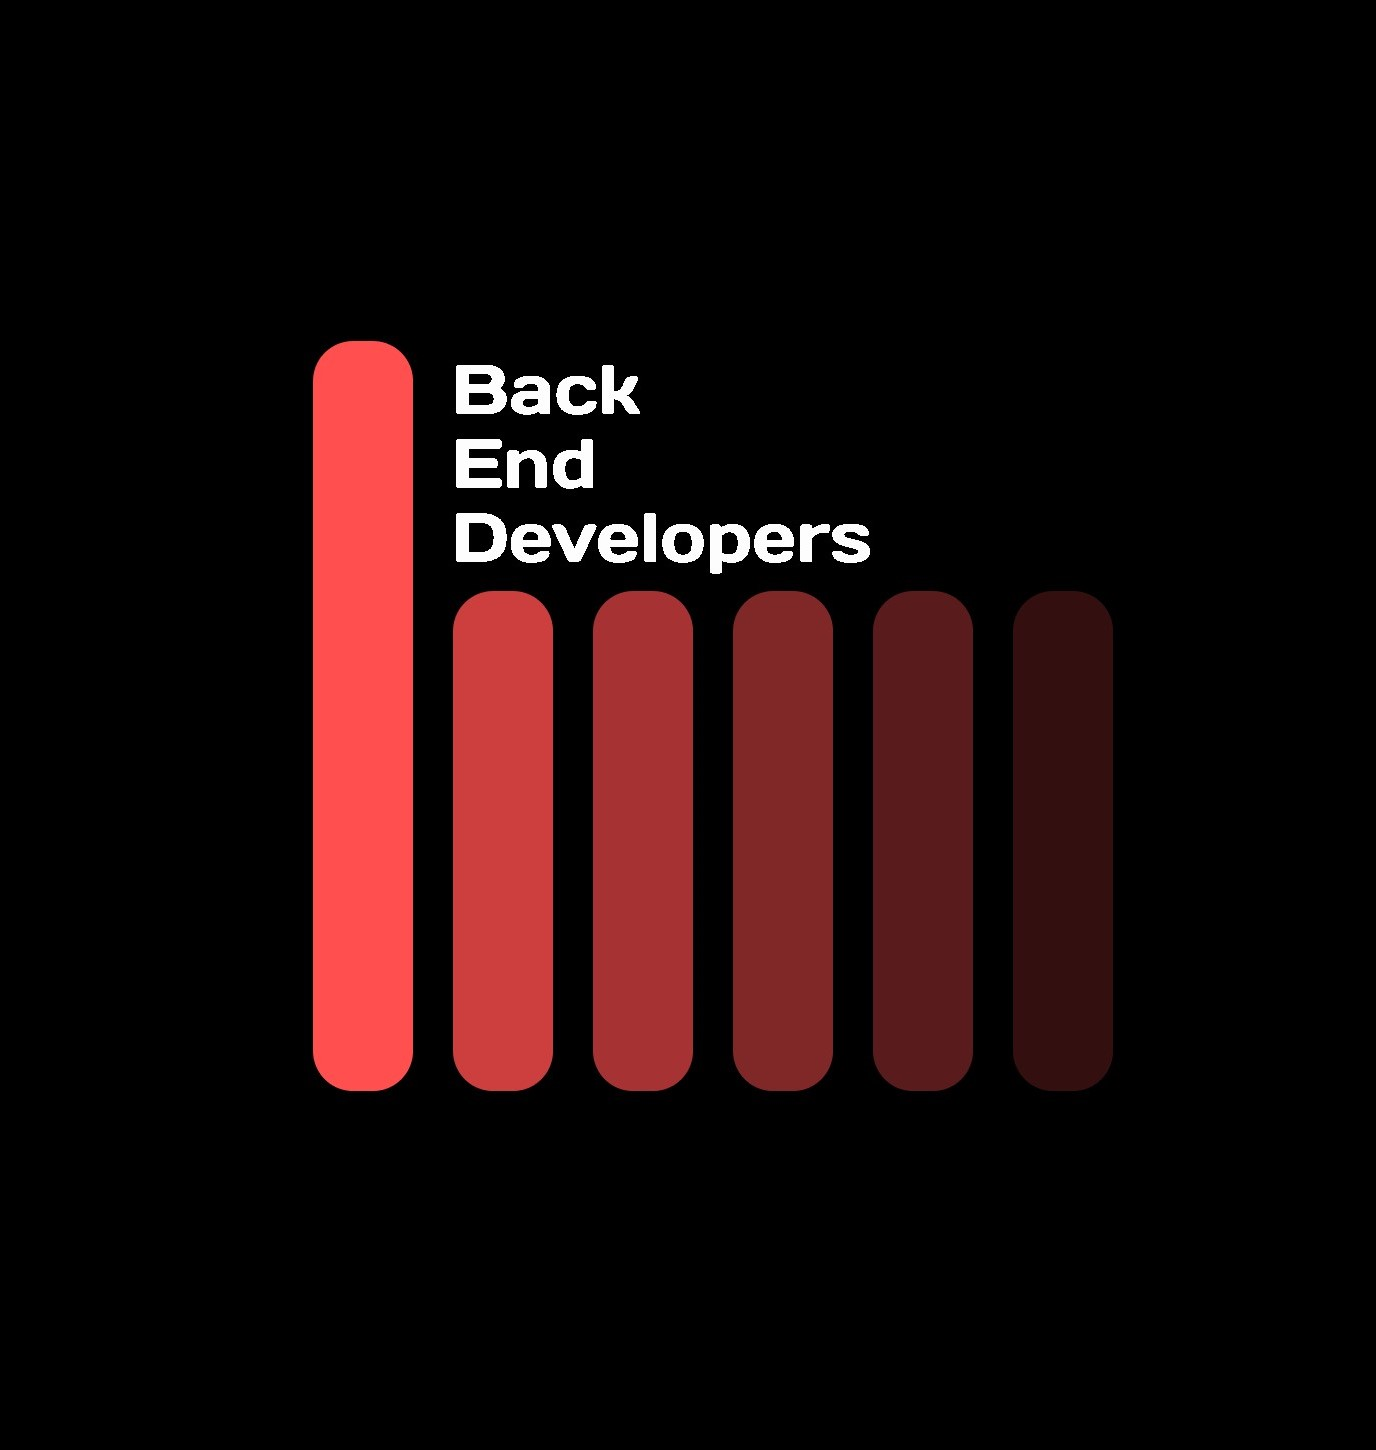
\includegraphics[width=0.5\textwidth]{../logo.jpg}}}
 \pagecolor{black}\afterpage{\nopagecolor}

\author{\authname}

\date{}

%% Comments

\usepackage{color}

\newif\ifcomments\commentstrue %displays comments
%\newif\ifcomments\commentsfalse %so that comments do not display

\ifcomments
\newcommand{\authornote}[3]{\textcolor{#1}{[#3 ---#2]}}
\newcommand{\todo}[1]{\textcolor{red}{[TODO: #1]}}
\else
\newcommand{\authornote}[3]{}
\newcommand{\todo}[1]{}
\fi

\newcommand{\wss}[1]{\authornote{blue}{SS}{#1}} 
\newcommand{\plt}[1]{\authornote{magenta}{TPLT}{#1}} %For explanation of the template
\newcommand{\an}[1]{\authornote{cyan}{Author}{#1}}

%% Common Parts

\newcommand{\progname}{ProgName} % PUT YOUR PROGRAM NAME HERE
\newcommand{\authname}{Team \#, Team Name
\\ Student 1 name and macid
\\ Student 2 name and macid
\\ Student 3 name and macid
\\ Student 4 name and macid} % AUTHOR NAMES                  

\usepackage{hyperref}
    \hypersetup{colorlinks=true, linkcolor=blue, citecolor=blue, filecolor=blue,
                urlcolor=blue, unicode=false}
    \urlstyle{same}
                                


\setlength\parindent{0pt}

\begin{document}

\color{white}\maketitle
\color{black}
\newpage
\begin{table}[hp]
    \caption{Revision History} \label{TblRevisionHistory}
    \begin{tabularx}{\textwidth}{llX}
        \toprule
        \textbf{Date}  & \textbf{Developer(s)} & \textbf{Change}       \\
        \midrule
        2022-09-26 &    Back End Developers   & Initial documentation \\
        2023-04-02 &    Jonathan Hai & Incorporated TA feedback \\
        2022-04-04 &    Jessica Bae & Added logo and style to the document \\
        \bottomrule
    \end{tabularx}
\end{table}

\newpage

\section{Problem Statement}

\subsection{Motivation Problem}

Dr. Luciana Macedo investigates treatment strategies for older adults with  lumbar spinal disorders (LSS), particularly focused on Ecological Momentary Assessment (EMA). EMA aims to study the thoughts, experiences, and behaviours of patients' daily lives by repeatedly collecting data in their day-to-day environment, at or close to the time they carry out that particular behaviour.\\

Since Dr. Macedo's EMA work is focused on analyzing the daily activities and symptoms of mostly-older adults with mobility issues, her solution needs to capture their slow and subtle movements. In order to accomplish this, she and her students have attempted to use various smart-watch-esque activity tracking devices along with various software applications to prompt their patients with questions. However, they have been frustrated with very limited success.\\

Their current system works on a time-based prompt-system, asking questions at regular intervals throughout the day. This is not as useful, as they are rather interested in the experiences of their patients when certain events or triggers happen. In addition, all of her data collection methods are heavily segregated and inefficient. In order to report their symptoms, a patient must input their answers into a smart watch, a mobile app, a website, etc. According to Dr. Macedo, this is not quite user-friendly especially when it comes to a group of older adult patients, and incredibly annoying and difficult for a researcher to analyze the gathered data. Importantly, the existing commercial products are designed to capture the activities of healthy and active people, which contrasts with what she is trying to capture: shuffling, limping, slower walking, etc.\\

The team at SReS requires a system which detects special (sometimes small-scale) movements from participants, relays prompts and information to participants based on said movements, and stores, analyzes, and displays movement data gathered throughout this process.\\


\pagebreak

\subsection{Inputs and Outputs}

\textbf{[Inputs]}
\begin{itemize}
    \item Sensors will detect relevant patient movement. Examples include:
	\begin{itemize}
		\item Limping
		\item Shuffling
		\item Foot-dragging
	\end{itemize}
    \item User responses to the survey for data collection.
\end{itemize}

\textbf{[Outputs]} \\
\linebreak
The output will be something that's useful for research and conclusion. This includes:
\begin{itemize}
    \item Graphically represented data.
    \item Specific numerical data of interest.
    \item Activity tracker for the user.
\end{itemize}

\subsection{Stakeholders}

Dr. Luciana Macedo of School of Rehabilitation Science at McMaster University.

\subsection{Environment}

Covered in the \href{https://github.com/zakerl/Capstone_Project/blob/main/docs/DevelopmentPlan/DevelopmentPlan.pdf}{Development Plan document}.
\newpage
\subsection{Constraints}
The constraints contained within this section were given by Dr. Luciana Macedo's research team. However, they may be subject to change according to the needs of the project and final product.
\begin{itemize}
    \item Safety: The device will be safe to use, with a voltage limit of 5V, and with adequate power protection circuitry in place.
    \item Weight: 100 grams. The device will be lightweight, so that it's portable and doesn't impact user's daily activities.
    \item Dimensions: 40mm long, and 34mm wide with a depth of 10.4 mm. A device of specified dimensions are very ergonomic and comfortable to wear.
    \item Accurate timing: System is very sensitive to timing inaccuracies, with no more than 1 minute of expected delay between detection and reporting.
    \item Battery Life: The device will be operable for a minimum of 24 hours without having to charge the device's battery.
    \item Data Retention for Period of EMA Study: Necessary storage for one EMA period's worth of data will be available within the device. This will provide the minimum amount of data storage necessary to enable EMA.
\end{itemize}

\pagebreak

\section{Base Goals}
\begin{center}
    \begin{longtable}{| m{2em} | m{7em} | m{16em}| m{14em} | }
        \hline
        \textbf{No.} & \textbf{Goal}                                    & \textbf{Explanation} & \textbf{Reasoning}                                                                                                                                                                                                                                                                                                                                                                                                                                                                                                                                                               \\
        \hline
       1) & Tacking Minor Movements                          & Most activity trackers make it difficult to track minor movements.
        They are generally created for highly mobile individuals such as athletes or similar. Since the target audience for this device will be older adults who have back and spinal problems; their movements will not be as pronounced as an athletes. & The tracker should have a good amount of sensitivity, so that minor movements like limping are appropriately accounted for.                                                                                                                                                                                                                                                       \\
        \hline
      2)  & Activity Based Prompting                            & The tracker should be able to prompt individuals when the activity monitoring system detects that a particular event has occurred, such as pausing after an activity has occurred.  Once prompted the individual will be asked to complete a Ecological Momentary Assessment (EMA) survey, in which they will be asked questions such as why they stopped moving, and if they are feeling any pain. & Having a visible prompting system that includes visual queues would be helpful in notifying participants that they should complete the EMA. This data will then be stored and used for further analysis. \\
        \hline
       3)& Simplistic User Interface and Hardware design &  It is essential that the design of the user interface and hardware be intuitive to a person without a lot of experience using smart technology. & The user base for this product will be the older adult population, some of whom may not use smartphones or smart watches. The product improves the likelihood that a user will fill out the survey successfully and quickly when prompted to do so.                                                                                                                                                                         \\
        \hline
       4) & Relevant \linebreak Presentation of Data                   & The data will be processed into an easy to interpret graphical or image based format that can be used to interpret the collected data. This will be displayed to the user to provide feedback on the activities that have been tracked throughout the day. & The researcher would view and collect data from the UI and will allow them to better understand the participant's movements and keep track of their rehabilitation programs. In addition, the option to export the raw data collected during the EMA period will be available, as well as the processed versions of the data.                                                                                                                                                                                      \\
	\hline
	5) & Customizeable Event Types and Thresholds			& Researchers will be able to customize the types of events that the device will detect and the thresholds that will activate them according to the needs of each individual EMA session and patient. Setting up the types of events to detect and their thresholds will be done before each monitoring period. The system will be configured in a way that will allow for a broad range of possible events to track, and will have many options to change properties of events and the types and levels of triggers for said events. & The configuration of the device needs to be changed by the researcher to fit each participant's requirements.
\\
        \hline
    \end{longtable}
\end{center}

\pagebreak

\section{Stretch Goals}
\begin{center}
    \begin{tabular}{ | m{2em} | m{7em} | m{16em}| m{12em} | }
        \hline
        \textbf{No.} & \textbf{Goal}                   & \textbf{Explanation} &  \textbf{Reasoning}                                                                                                                                                                                                                                                                                                                                                           \\
        \hline
        1) & Anomaly \linebreak Detection               & The device should detect when certain anomalies occur. Some examples include: an abrupt stop in movement and then a prolonged duration of no movement (indicated a potential accident), major spikes in movements (sudden increases in acceleration, speed or, orientation changes), or other abnormal events. & Detecting anomalies would improve user safety and quality of data collection. \\
        \hline
      2) &   Geo-tagging Events and Movements & Geo-tracking users and movements could show if majority of activity is closer to home or away from home. &  This data will enable better primary data collection and help understand how users movements change throughout the day in a location and time based manner.                                                                                                  \\
        \hline
      3) &   Movement based-charging system  & Having a system that charges using movement could be beneficial to users and help extend usable time. & This would mean less charging and greater convenience. As part of this goal, reducing power draw would be an important aspect to make the movement based charging worthwhile.                                                                                                            \\
        \hline
    \end{tabular}
\end{center}


\end{document}